\documentclass{article}
\usepackage{amssymb,amsmath}
\usepackage{ifxetex,ifluatex}
\ifxetex
  \usepackage{fontspec,xltxtra,xunicode}
  \defaultfontfeatures{Mapping=tex-text,Scale=MatchLowercase}
\else
  \ifluatex
    \usepackage{fontspec}
    \defaultfontfeatures{Mapping=tex-text,Scale=MatchLowercase}
  \else
    \usepackage[utf8]{inputenc}
  \fi
\fi
\usepackage{ctable}
\usepackage{float} % provides the H option for float placement
\usepackage{graphicx}
% We will generate all images so they have a width \maxwidth. This means
% that they will get their normal width if they fit onto the page, but
% are scaled down if they would overflow the margins.
\makeatletter
\def\maxwidth{\ifdim\Gin@nat@width>\linewidth\linewidth
\else\Gin@nat@width\fi}
\makeatother
\let\Oldincludegraphics\includegraphics
\renewcommand{\includegraphics}[1]{\Oldincludegraphics[width=\maxwidth]{#1}}
\ifxetex
  \usepackage[setpagesize=false, % page size defined by xetex
              unicode=false, % unicode breaks when used with xetex
              xetex]{hyperref}
\else
  \usepackage[unicode=true]{hyperref}
\fi
\hypersetup{breaklinks=true, pdfborder={0 0 0}}
\setlength{\parindent}{0pt}
\setlength{\parskip}{6pt plus 2pt minus 1pt}
\setlength{\emergencystretch}{3em}  % prevent overfull lines
\setcounter{secnumdepth}{0}

\title{example script}
\author{(Username not set) (E-mail address not set)}
\date{2011--04--26 20:25 CET}

\begin{document}
\maketitle

\subsection{Description}

A simple report.

\subsubsection{Descriptive statistics}

The average fuel consumption is 20.091 with SD of 6.0269. Let's add one
more line to this paragraph. And another one. Now, you've probably heard
of \emph{pi}? Right? Its value is 3.1416.

\subsubsection{Graphs}

And some graphs:

\begin{figure}[htbp]
\centering
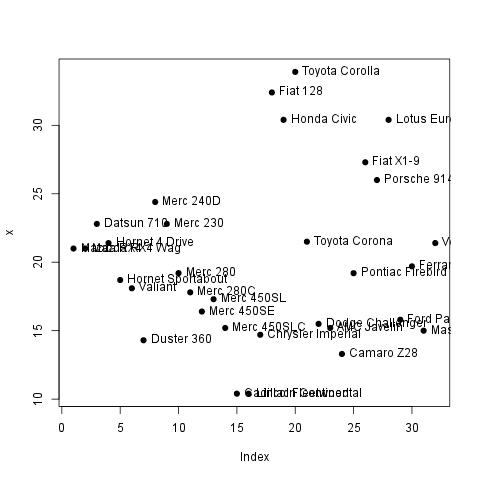
\includegraphics{0ec1f788fe2feb5d233de865b51e9eaf.png}
\caption{}
\end{figure}

So far we've been dealing with data.frames and plots, now let's deal
with variables

Now we'll see if the Z var is working properly. If I omit it, it should
perserve the default value (TRUE)\ldots{} aaaand\ldots{}. TRUE.

OK, so far, so good, but let's see what's going on with code
chunks\ldots{}

\ctable[pos = H, center, botcap]{llllllllll}
{% notes
}
{% rows
\FL
--0.7233 & 0.4846 & 1.1837 & --1.1286 & 0.7626 & --0.2007 & 0.8247 & 2.0190 & --1.1185 & 0.2930
\\\noalign{\medskip}
--0.4760 & 0.3876 & --1.3727 & --0.7365 & --0.5195 & --0.5273 & --0.8474 & 0.8597 & 1.2813 & --0.9687
\\\noalign{\medskip}
--1.1426 & --0.5208 & 0.1674 & 1.6176 & --0.4365 & --0.8570 & --1.2663 & 0.0950 & 1.2360 & 0.0432
\\\noalign{\medskip}
2.5510 & --1.9335 & 0.7801 & 0.5611 & 0.8377 & --0.6773 & 1.0799 & --0.3940 & --0.7981 & --1.1803
\\\noalign{\medskip}
0.2170 & 0.5017 & 0.2235 & --2.4930 & 0.8394 & 0.9265 & 0.1297 & 0.2896 & 2.4994 & 0.7075
\\\noalign{\medskip}
--0.0047 & --0.4469 & 0.6343 & 0.1612 & 0.1363 & --1.6824 & --0.7752 & 0.0451 & --2.1691 & --1.3664
\\\noalign{\medskip}
--0.6078 & --0.4940 & --0.7693 & 1.1545 & --0.2569 & 1.1001 & --2.0265 & --0.1971 & 0.2023 & --1.4957
\\\noalign{\medskip}
0.1597 & --0.1338 & --0.0163 & --0.6640 & --1.3500 & 0.2761 & --1.5970 & --0.9246 & 1.2280 & 0.8607
\\\noalign{\medskip}
0.8559 & 1.9824 & 0.8633 & --0.5892 & --2.0797 & 0.3542 & --0.2304 & 0.5624 & --0.4461 & 0.4142
\\\noalign{\medskip}
0.4493 & --3.0249 & 0.1643 & --0.6460 & 1.0125 & --1.2532 & 0.0074 & 0.0643 & 0.3017 & 0.0577
\LL
}

When it comes to CSV values, let us see how do they work. You have
chosen the ``foo''.

\subsection{Description}

A simple report.

\subsubsection{Descriptive statistics}

The average fuel consumption is 146.69 with SD of 68.563. Let's add one
more line to this paragraph. And another one. Now, you've probably heard
of \emph{pi}? Right? Its value is 3.1416.

\subsubsection{Graphs}

And some graphs:

\begin{figure}[htbp]
\centering
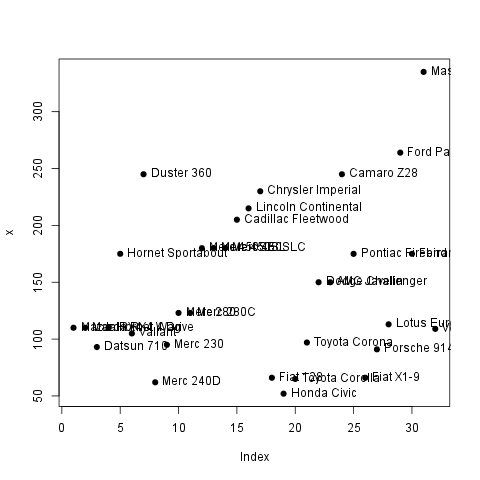
\includegraphics{0221aa97b1343432a8450115ebf9089f.png}
\caption{}
\end{figure}

So far we've been dealing with data.frames and plots, now let's deal
with variables

Now we'll see if the Z var is working properly. If I omit it, it should
perserve the default value (TRUE)\ldots{} aaaand\ldots{}. TRUE.

OK, so far, so good, but let's see what's going on with code
chunks\ldots{}

\ctable[pos = H, center, botcap]{llllllllll}
{% notes
}
{% rows
\FL
--0.3962 & --1.5590 & 3.4704 & 1.3368 & 0.2663 & --0.1400 & 0.4214 & --0.1471 & --0.9187 & --1.7328
\\\noalign{\medskip}
--0.6559 & --1.0874 & --0.6273 & 0.5882 & --1.5250 & --0.6167 & 0.0354 & --0.8753 & 0.4180 & --0.4941
\\\noalign{\medskip}
--0.4818 & --0.1483 & --0.0883 & --1.6596 & 0.3462 & 0.5981 & 0.1383 & 0.6230 & 0.7428 & 0.7190
\\\noalign{\medskip}
0.2829 & --0.6523 & --0.7189 & --2.8530 & 0.0879 & --0.3051 & --1.7278 & 0.7643 & 1.7792 & 1.0526
\\\noalign{\medskip}
0.2223 & 0.6517 & 1.3913 & 0.9833 & --0.5834 & --0.9909 & --0.4537 & --0.6580 & 2.3794 & 2.0675
\\\noalign{\medskip}
--0.3149 & --0.8477 & --0.5503 & 0.9162 & --0.1697 & 1.2714 & 0.4634 & --0.1064 & --0.1837 & --0.2410
\\\noalign{\medskip}
0.0710 & 0.0065 & --0.3533 & 0.8112 & 0.1743 & --0.1558 & --0.1437 & 1.0345 & --0.1120 & 0.7749
\\\noalign{\medskip}
0.8539 & --1.7140 & 0.5383 & 0.2295 & 0.3292 & --0.3990 & 1.0702 & --1.1600 & --0.0425 & 0.9982
\\\noalign{\medskip}
1.8481 & --1.9760 & 1.9041 & 0.2946 & --0.2601 & 0.0581 & --1.3820 & 0.5470 & --0.0525 & 0.2462
\\\noalign{\medskip}
--0.7469 & 1.5056 & --0.1318 & 1.6810 & 1.2991 & 0.2174 & 0.8966 & 0.0914 & --0.3156 & 0.9390
\LL
}

When it comes to CSV values, let us see how do they work. You have
chosen the ``foo''.

\subsection{Description}

A simple report.

\subsubsection{Descriptive statistics}

The average fuel consumption is 2.0628 with SD of 2.0404. Let's add one
more line to this paragraph. And another one. Now, you've probably heard
of \emph{pi}? Right? Its value is 3.1416.

\subsubsection{Graphs}

And some graphs:

\begin{figure}[htbp]
\centering
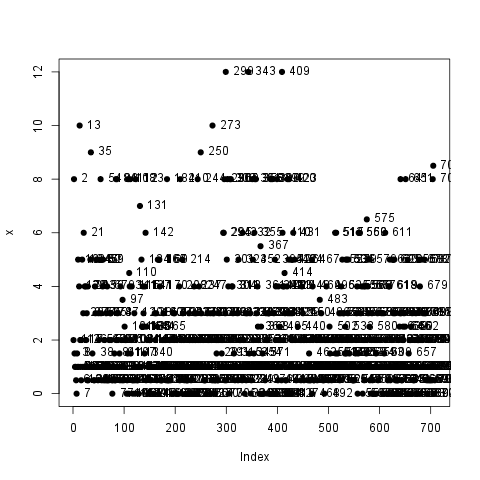
\includegraphics{f1891776819c845a6068c59a90f70d8f.png}
\caption{}
\end{figure}

So far we've been dealing with data.frames and plots, now let's deal
with variables

Now we'll see if the Z var is working properly. If I omit it, it should
perserve the default value (TRUE)\ldots{} aaaand\ldots{}. TRUE.

OK, so far, so good, but let's see what's going on with code
chunks\ldots{}

\ctable[pos = H, center, botcap]{llllllllll}
{% notes
}
{% rows
\FL
1.5299 & --0.2729 & 2.1052 & --1.9148 & --0.2537 & 0.3264 & 1.3741 & --0.3369 & 0.8517 & 0.0286
\\\noalign{\medskip}
0.9124 & --0.0866 & 0.2420 & --0.5868 & --1.1475 & --1.7872 & --0.1422 & --1.7004 & 1.1141 & --1.0209
\\\noalign{\medskip}
0.9227 & --1.1400 & 0.3641 & 0.1442 & 0.6264 & 1.8114 & 0.1281 & 0.4555 & 1.2501 & 0.6140
\\\noalign{\medskip}
--0.1787 & --0.8168 & 1.1941 & 0.9664 & 0.8456 & --0.4854 & 0.3648 & 0.7771 & --1.6458 & 0.2871
\\\noalign{\medskip}
1.7283 & 0.0090 & --0.4299 & --0.4292 & --0.3123 & 0.8632 & --0.7604 & 0.7302 & --1.2917 & 0.4755
\\\noalign{\medskip}
0.7234 & 1.4822 & --0.5963 & 0.1039 & 0.5531 & --0.4504 & --2.0211 & --0.5702 & 0.7103 & 1.1360
\\\noalign{\medskip}
1.2239 & 0.1094 & 0.3881 & --0.5168 & 1.7920 & --0.1848 & 0.4061 & --0.2263 & 1.3268 & --1.7374
\\\noalign{\medskip}
0.3648 & 2.3190 & 0.6969 & 0.5445 & 0.7666 & --1.2162 & --0.3891 & 0.4663 & --0.0411 & --1.8405
\\\noalign{\medskip}
--1.2790 & 0.7390 & --0.5244 & --1.0051 & 2.1517 & --0.9225 & --0.3475 & 0.9721 & 0.0728 & 1.8239
\\\noalign{\medskip}
0.0528 & 0.4392 & 0.0117 & 0.1516 & --1.5187 & --2.0555 & --0.5169 & --0.2793 & --0.2679 & 0.9850
\LL
}

When it comes to CSV values, let us see how do they work. You have
chosen the ``foo''.

\end{document}
